
\chapter{Quantifying G.U. Filtering on Toy Experiment}
\label{ch:quantifying_gu_filtering_toy}

In \cite{jazbec_generative_2025}, the toy experiment was used to demonstrate the effectiveness of \acs{GU} on the very simple mixture of gaussian dataset. Although it was visually very convincing, we will go deeper into what the filtering actually does.

\begin{tcolorbox}[colback=orange!10!white,colframe=orange!50!black,sharp corners]
It should be noted that we are still using a Deep Ensemble (\acs{DE}) instead of a \acs{LA} to get the $\text{M}+1$ models used for uncertainty quantification. We describe here how that \acs{DE} Uncertainty behaves and in \autoref{ch:toy_exp_posterior} we switch to a \acs{LA} based Ensemble and highlight major behavioral differences.
\end{tcolorbox}

\section{Metrics}
\label{sub:toy_metrics}

We start by defining a couple of metrics to quantify if filtering the generated dataset brings it closer to the reference distribution. We are essentially trying to get an equivalent to the \acs{FPR} metrics for the toy experiment.

\subsection{Log-Likelihood}

We know the analytical form of the reference distribution, we can easily evaluate the likelihood of a point $x \in \mathbb{R}^2$ being part of this dataset.

\begin{equation}
\label{eq:log-lik-toy}
p(x) = \frac{1}{25} \sum_{i=1}^{25} \mathcal{N}(x | \mu_i,\sigma^2 I)
\end{equation}


To safely (avoid underflow) sum/combine the 25 gaussian probabilities of $p(x)$, we use \texttt{scipy.special.logsumexp}.

\begin{equation}
\log p(x) = \log \left( \frac{1}{25} \sum_{i=1}^{25} \exp \Big( \log \mathcal{N}(x \ | \ \mu_i, \sigma^2 I) \Big) \right)
\end{equation}


The log-likelihood for the whole dataset is simply:
\begin{align}
    \log p(\mathcal{D}) = \sum_{x \in \mathcal{D}} \log p(x)
\end{align}

Where $\mathcal{D}$ is either the full generated dataset or a selected subset obtained by filtering.
% We wish to obtain the log likelihood $\log P(\textbf{x}) = \sum \log P(x)$, $x \in \text{D}_{\text{generated | filtered}}$.

The log-likelihood gives us an idea of the precision of the generated dataset. The closer the points are to the modes, the higher their probability. However, this metric cannot quantify diversity. For instance if we had a model that assigned all $x$ to the center of single mode $\mu_j$, it would maximize the likelihood while poorly representing the reference distribution.
To fix this, we introduce a KL Divergence metric.

\subsection{KL Divergence}
To quantify diversity, specifically whether all 25 modes are covered equally, we evaluate the divergence at the mode assignment level using the discrete Kullback-Leibler (KL) divergence:

$$D_{KL}(P || Q)=\sum_{i=1}^{25}P(i)\log\left(\frac{P(i)}{Q(i)}\right)$$

Here, $Q(i)=1/25$ represents the ideal uniform coverage from the reference distribution. We compute the empirical coverage fraction $P(i)$ by assigning each generated point to its closest mode center ($\mu_i$) based on the minimum Euclidean distance ($L_2$ norm), counting them and dividing by the total number of generated points.

While this successfully captures inter-mode coverage, it ignores intra-mode variance (e.g., if a model perfectly balances mode assignments but unnaturally clusters points exactly at the centers). To measure this spread, we introduce a direct per-mode (intra-)variance metric.

\subsection{Direct per Mode Variance}

First, just like before we assign each generated sample to its closest mode. Then for each mode we compute its variance across its associated generated samples. We then take the average (avg) across the modes of the per mode variance ($\hat{\sigma}_{avg}^2 = \text{average empirical variance}$) and compare it to the reference distribution's mode variance $\sigma^2$ via a variance ratio $r=\frac{\hat{\sigma}_{avg}^2}{\sigma^2}$.

\subsection{Maximum Mean Discrepancy (MMD)}

As a final, more conventional metric, we use the Maximum Mean Discrepancy (\acs{MMD}), which compares the two distributions as a whole instead of isolating a single aspect. It relies on a kernel $k(x,y)$ measuring the similarity between two points. Given samples $X \sim P$ and $Y \sim Q$, the squared \acs{MMD} compares the average within-set similarities to the average cross-set similarity:

\begin{equation}
\text{MMD}^2(X, Y) = \mathbb{E}[k(x, x')] + \mathbb{E}[k(y, y')] - 2\,\mathbb{E}[k(x, y)],
\end{equation}
which is zero exactly when $P$ and $Q$ are indistinguishable under the kernel. We use the standard Radial Basis Function (RBF) kernel $k(x,y) = e^{-\gamma \|x-y\|^2}$ directly on the raw 2D points (unlike \acs{FID}, no learned embedding is needed here). Its only parameter $\gamma$ sets the length scale at which two points count as similar. The usual median heuristic, $\gamma = \tfrac{1}{2M}$ with $M$ the median of the \emph{squared} pairwise distances, is here dominated by the large inter-mode distances and gives too wide a kernel; we therefore set $\gamma = 0.2$ by hand to stay sensitive to intra-mode structure as well.

\subsection{Drawing the Parallel}

We can end this section by drawing parallels between the \acs{FPR} metrics and the metrics defined here.
\begin{itemize}
    \item Log-Likelihood can be thought of as an equivalent for \emph{Precision}.
    \item KL Divergence and Direct Per Mode Variance together can be seen as an equivalent for \emph{Recall}.
    \item \acs{MMD} can be seen as the equivalent for \acs{FID}.
\end{itemize}

\section{Metrics Results}

Now let's use the metrics we just defined, and try to explain how filtering with Deep Ensemble (\acs{DE}) based \acs{GU} affects the resulting dataset.

\begin{figure}[!htbp]
    \centering
    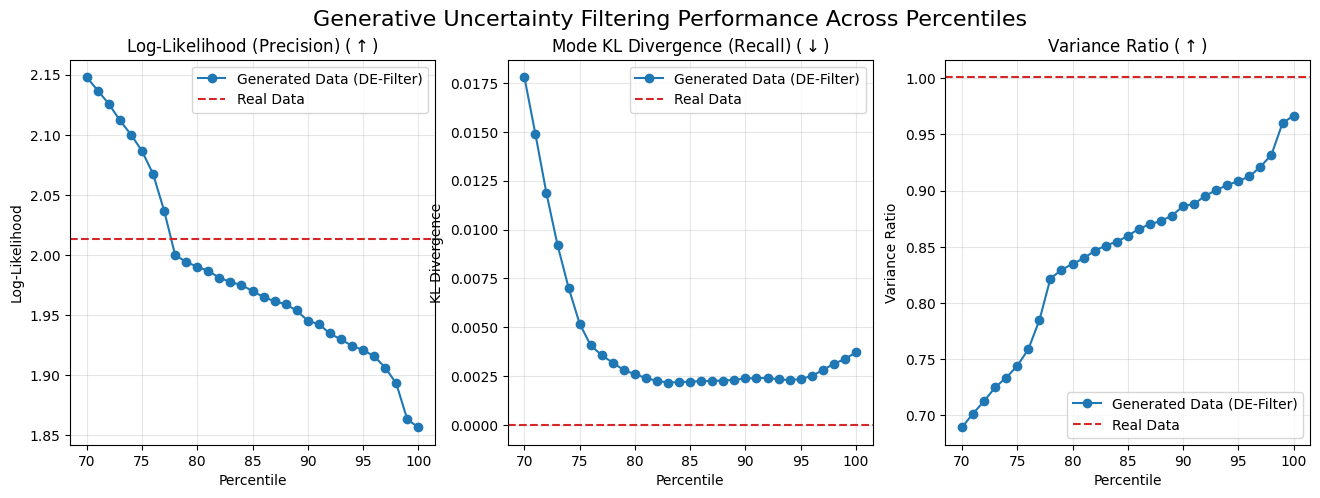
\includegraphics[width=0.95\linewidth]{figures/toy_experiment/de_gmm_perf.png}
    \caption{Performance of the filtering across 3 metrics: Log-Likelihood, KL Divergence and Variance Ratio}
    \label{fig:toy_gmm_perf_de}
\end{figure}

With \autoref{fig:toy_gmm_perf_de}, we observe that the benefits of filtering out bad samples stops abruptly around the 77th percentile at which point the KL Divergence and Variance ratio worsen at a very quick rate while log-likelihood explodes. This sudden rise of likelihood could be explained by the filtering metric being done with actual out of distribution samples and starting to eat through valid samples that are further to the mode centers $\mu_j$.

\begin{figure}[!htbp]
    \centering
    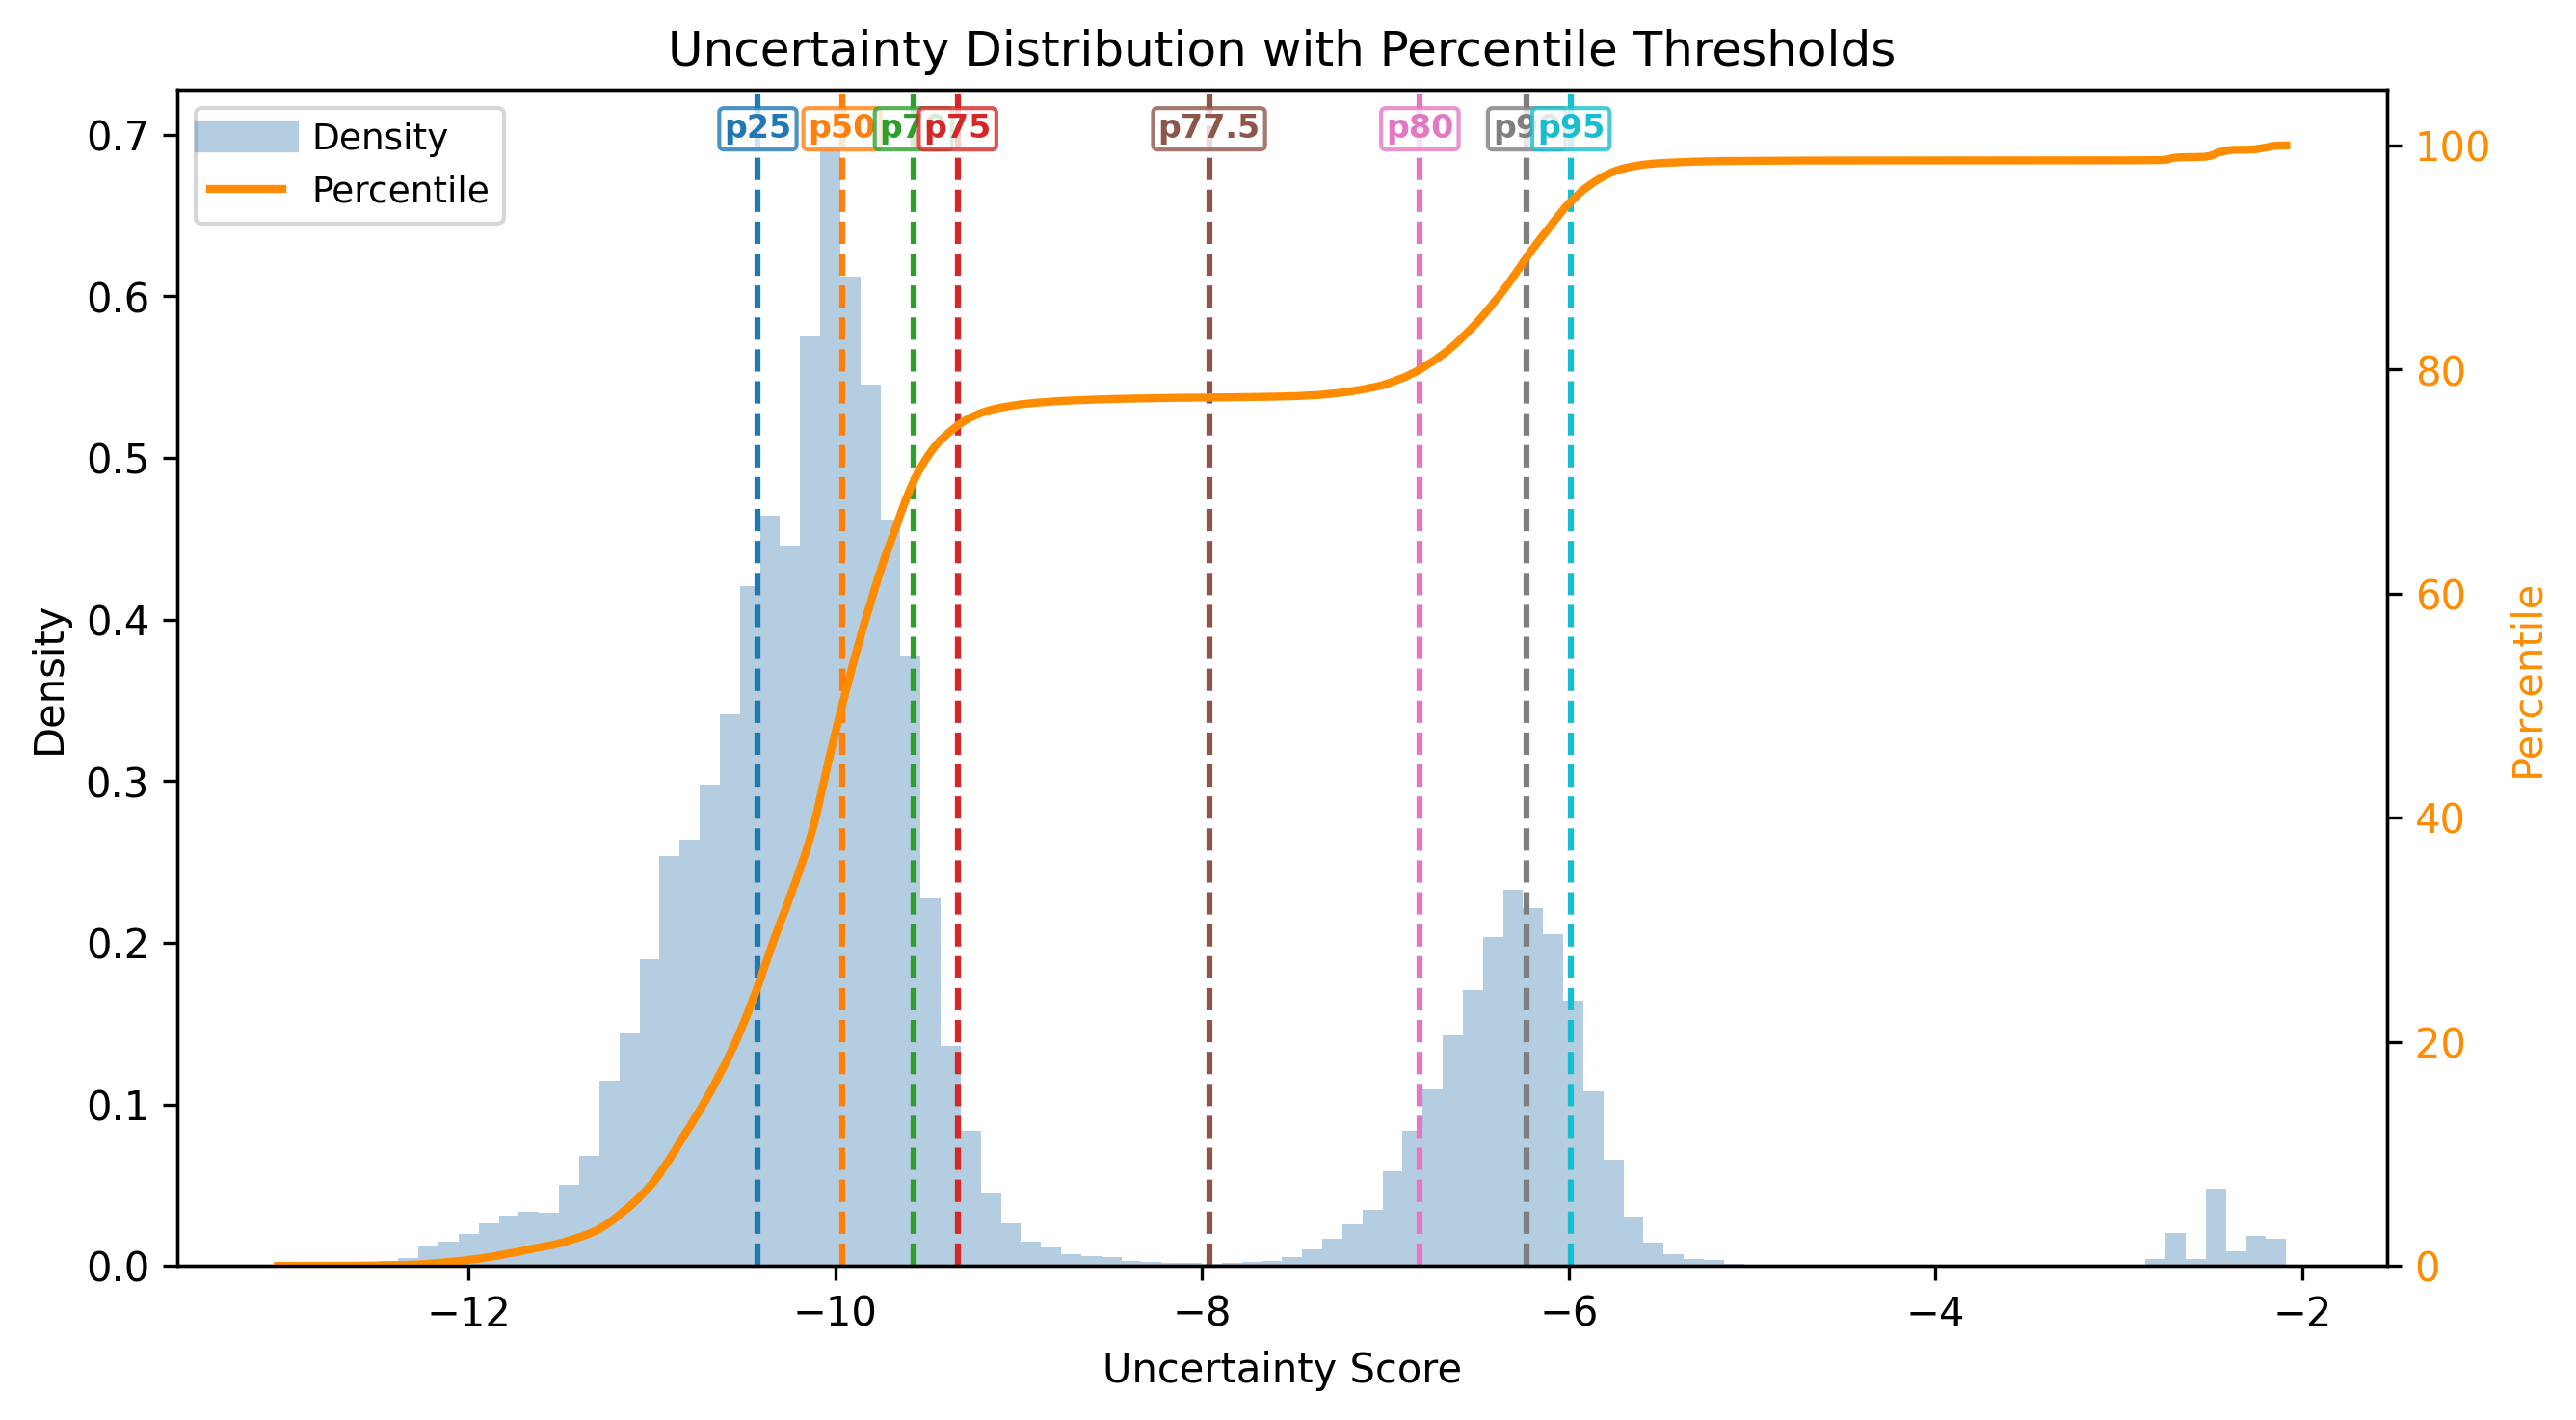
\includegraphics[width=0.8\linewidth]{figures/toy_experiment/uncertainty_dist.png}
    \caption{Uncertainty Distribution Histogram (Lower is better). This plot helps to visualize what part of the uncertainty in the samples the percentile threshold is actually removing. A threshold of 80 means that we keep $80\%$ of the samples (located at the left of the threshold).}
    \label{fig:toy_uncertainty_dist}
\end{figure}

We can draw an histogram of the uncertainty scores distribution to get more insight (\autoref{fig:toy_uncertainty_dist}) and see that our observation is perfectly matched by a tail of uncertainty located above the 77th percentile (\textcolor{brown}{$p77.5$}).

We can now also look at a scatter plot of the filtered datasets at different percentiles to confirm what we observed in the metrics and histogram. We see in \autoref{fig:toy_filtered_data} that $77\%$ is indeed the sweet spot. Just above ($80\%$), we still have some obvious hallucinations. At $70\%$, we start to significantly reduce the size of some mode (intra-mode variance) non-uniformly across all modes (inter-mode).

\begin{figure}[!htbp]
    \centering
    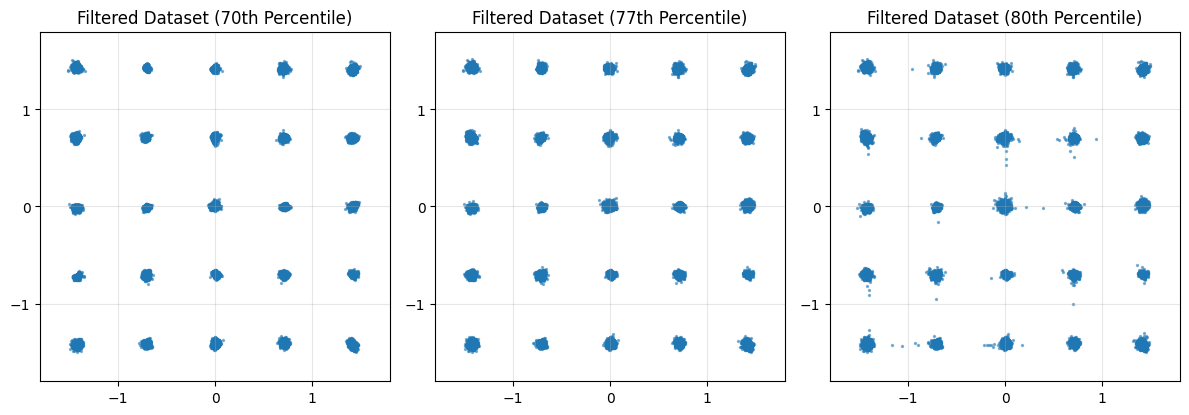
\includegraphics[width=0.9\linewidth]{figures/toy_experiment/toy_filtered_data.png}
    \caption{Deep Ensemble (DE) Generative Uncertainty (GU) Filtered Samples at a percentiles of $70\%, 77\%, 80\%$}
    \label{fig:toy_filtered_data}
\end{figure}

Finally, we can also take a look at the MMD metric (\autoref{fig:toy_mmd}), to add a more general metric to what we already have. Although the estimation of MMD is quite unstable (large confidence intervals), we still see the explosion in the $75-80$ range.

\begin{figure}[!htbp]
    \centering
    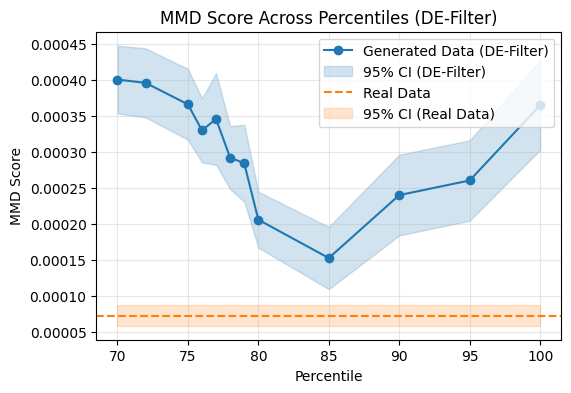
\includegraphics[width=0.6\linewidth]{figures/toy_experiment/mmd_score.png}
    \caption{\acs{MMD} metric across percentiles}
    \label{fig:toy_mmd}
\end{figure}

\section{What Does Deep Ensemble based Generative Uncertainty Filter Out?} 
\label{sec:toy_what_gu_filter}

When looking at the generated dataset (\autoref{fig:toy_data}), it does not really look like as much as $23{,}000$ ($23\%$ of $100{,}000$) points are inter-mode hallucinations. 

In this section, we try to get an idea of what points are actually being filtered out by the Deep Ensemble based Generative Uncertainty.

We define ``hallucination'' as a point $\boldsymbol{x}$ for which the distance to the closest mode is bigger than $6\sigma$ with $\sigma$ being the standard deviation of a mode. If we assume that the filtering metric should target ``hallucinations'', we can define 4 buckets to sort the generated points after filtering into:

\begin{itemize}
    \item \textcolor{Cerulean}{Rightfully Kept} (\textbf{TN}): The points that were not filtered out and are not ``hallucinations''.
    \item \textcolor{Green}{Rightfully Caught} (\textbf{TP}): points that were filtered out and are ``hallucinations''
    \item \textcolor{orange}{Wrongfully Shaved Halos} (\textbf{FP}): points that were filtered out but weren't ``hallucinations''
    \item \textcolor{red}{Missed Hallucinations} (\textbf{FN}): points that were not filtered out but were ``hallucinations''
\end{itemize}

\begin{figure}[!htbp]
    \centering
    \begin{subfigure}[b]{0.45\textwidth}
        \centering
        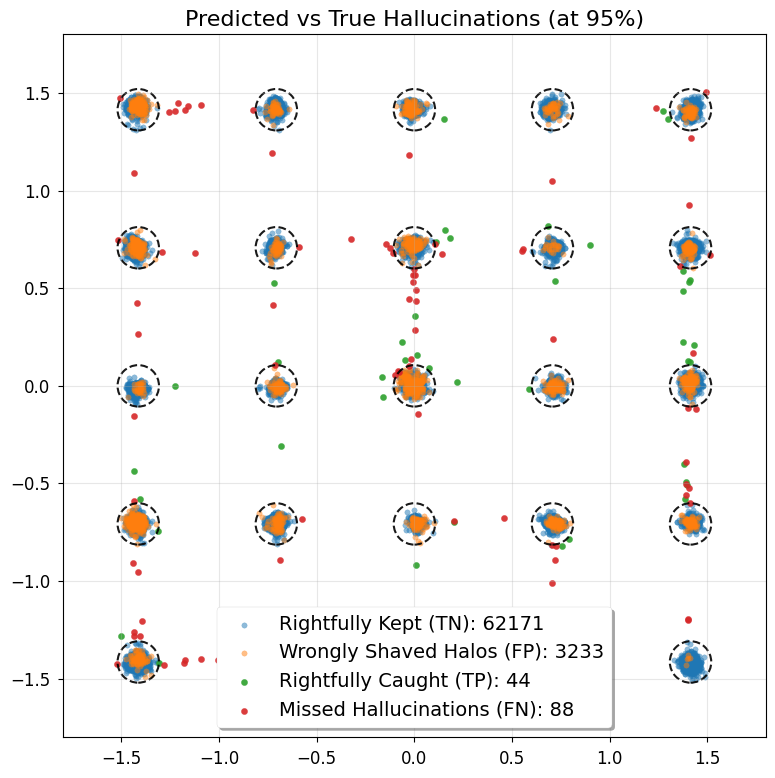
\includegraphics[width=\textwidth]{figures/toy_experiment/where_hallucinations.png}
        \caption{Visualizing what deep uncertainty is filtering at $95\%$ ($r=5\%$) by splitting the generated samples into the 4 buckets}
        \label{fig:where_hallucinations}
    \end{subfigure}
     % \hfill
    \begin{subfigure}[b]{0.45\textwidth}
        \centering
        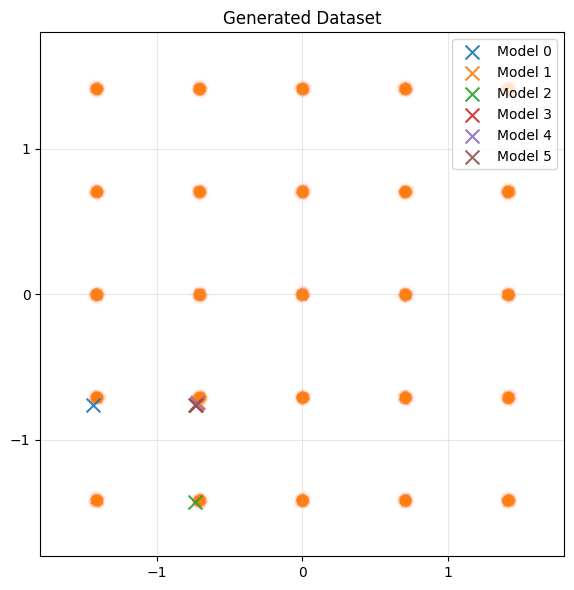
\includegraphics[width=\textwidth]{figures/toy_experiment/sample_accross_models.png}
        \caption{One of the most uncertain points from the \acs{GU} metric shown across the $\text{M}+1$ models, displayed on top of the reference dataset}
        \label{fig:sample_accross_models}
    \end{subfigure}
    \caption{\acs{DE} Hallucinations Analysis}
    % \caption{Taking the 4 most and least uncertain (w.r.t. \acs{GU}) images in a dataset 12032 generated images}
    \label{fig:hallucinations_where_how_much}
\end{figure}

Drawing those buckets in a scatter plot of the filtered samples at the 95th percentile gives us \autoref{fig:where_hallucinations}. We see that the filtered points are actually dominated by \textbf{FP}s (3233 \textbf{FP}s for 44 \textbf{TP}s despite missing 88 \textbf{FN}s). Either \acs{DE} based uncertainty is really bad at filtering out ``hallucinations'' or it is filtering something more.

This leads us to investigate why those \textbf{FP} points have such a high uncertainty despite being located so close to a mode and being a seemingly valid sample. \autoref{fig:sample_accross_models} represents a very high uncertainty sample classified as \textbf{FP}. It is shown across the $1+\mathrm{M} = 6$ models. We immediately understand why we get so many \textbf{FP}s, despite each model producing a valid sample with respect to the reference distribution, the same starting noise $z$ lead to generated samples being assigned to different modes, leading to very high uncertainty.

\paragraph{Conclusion}
We can conclude from this experiment that uncertainty is not limited to ``hallucinations'' as we defined them. Uncertainty also targets samples where the model was unsure which mode to assign to.
% We therefore have to define uncertain points as something different from the current definition of hallucinations we have. Uncertainty is a broader concept and is also targeting starting noise for which the model was unsure which mode to assign to.

Measuring how well generative uncertainty performs on the toy dataset with respect to this broader definition of uncertainty is a much harder task, samples like \autoref{fig:sample_accross_models} are valid for each model taken individually but highly uncertain when comparing the output between models.
For the remainder of our experiment, we will simply define the \acs{DE} based Generative Uncertainty as the source of truth for uncertainty. In the next chapter, we compare the much cheaper ways to get the \acs{MC} ensemble of models (\acs{LA}) against the (\acs{DE}).

%%%%%%%%%


\chapter{Refining the Posterior Approximation with the Toy Experiment}
\label{ch:toy_exp_posterior}

\vspace{20pt}

Until now, we have approximated the posterior distribution using \acs{DE}. For large models like \acs{ADM}, training $\mathrm{M}$ additional models to get a \acs{DE} is computationally prohibitive. While late epoch checkpoints or extended training offer alternatives, they remain costly. Following \cite{jazbec_generative_2025}, we focus on the efficient, \textbf{post-hoc} application of \acs{GU} to pretrained models.

\begin{figure}[!htbp]
    \centering
    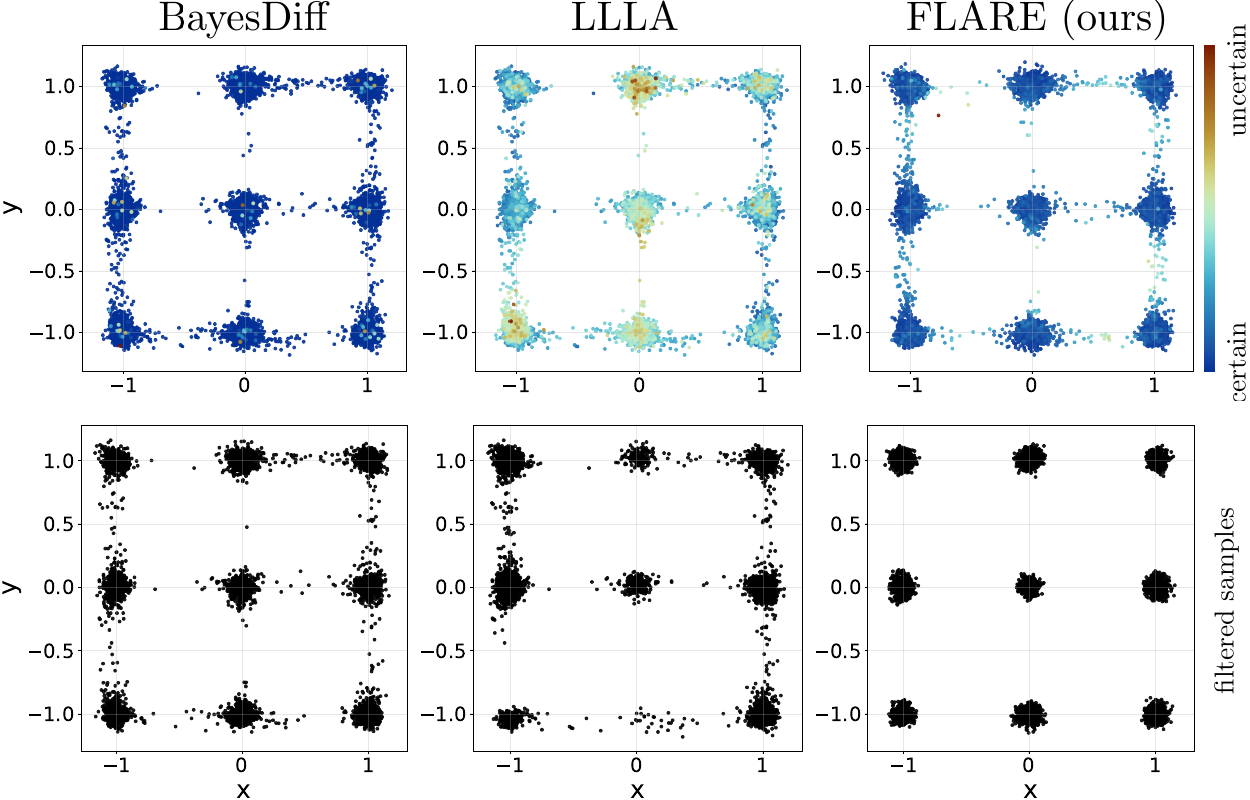
\includegraphics[width=0.7\linewidth]{figures/extend_toy/gupta_mixture.png}
    \caption{Taken from \cite{gupta_quantifying_2026}, a reproduction of \parencite{aithal_understanding_2024, jazbec_generative_2025} experiment with a 9-mode gaussian mixture. BayesDiff, \acs{LLLA} and FLARE are displayed as methods of computing the uncertainty. On the top we see the uncertainty heatmap for each generated samples, on the bottom we see the remaining samples after filtering.
    \warning FLARE is \cite{gupta_quantifying_2026} method that supposedly fixes flaws from \cite{jazbec_generative_2025} including sampling the uncertainty throughout the whole diffusion process and improving the posterior approximation. \acs{LLLA} here is the FLARE method without the improved posterior approximation, which is therefore not the same as the \acs{LLLA} method we define in \autoref{ch:gu_theory}.}
    \label{fig:gupta_mixture_llla_flare}
\end{figure}

Furthermore, \cite{jazbec_generative_2025} uses \acs{DE} for their \textit{Toy Experiment} but switches to a Last Layer Laplace Approximation (\acs{LLLA}) for the \acs{ADM} experiment, without evaluating the \acs{LLLA} on the toy dataset. This omission is worrying given that \autoref{fig:gupta_mixture_llla_flare} (from \cite{gupta_quantifying_2026}) shows an \acs{LLLA} based method performing poorly in a setting close to the Toy experiment.

Thankfully, this chapter will demonstrate that when properly stabilized (prior and temperature), the \acs{LLLA} can effectively filter parts of the uncertainty\footnote{As we've seen in the previous chapter, uncertainty is more than just ``hallucinations''} well, even significantly outperforming Deep Ensembles when it comes to filtering ``hallucinations'' specifically.

\section{Last Layer Laplace Approximation} 

To apply the \acs{LLLA} to the Toy experiment, we essentially use the method defined in \autoref{ch:gu_theory} without the semantic encoder (not needed when working with points in 2D). In summary: The \acs{LLLA} uses the Empirical \acs{FIM} with a diagonal factorization to approximate the Hessian. Assuming an isotropic Gaussian prior $\theta \sim \mathcal{N}(0, \gamma^{-1}I)$, we get the \acs{LLLA} of the posterior as $q(\theta|\mathcal{D})=\mathcal{N}(\theta;\hat\theta, \Sigma_\theta)$ with $\hat\theta$ the pretrained \acs{MLE} model and $\Sigma_\theta = H^{-1} = (\nabla^2_\theta N\mathcal{L}_{\mathrm{simple}}(\theta)|_{\hat\theta} + \gamma I)^{-1}$ in this expression, we name the first term ``Hessian of the \acs{NLL} (Negative Log-Likelihood)'' and second ``Hessian of the Negative Log Prior''.

The prior $\gamma$ regularizes the covariance matrix, preventing extreme values along flat directions of the Hessian $H$.

% We evaluate the Laplace Approximation (LA) against the Deep Ensemble (DE) baseline via an 

\paragraph{Ablation Study on $\gamma$}
We first conduct an ablation study on $\gamma \in [0.01; \dots; \allowbreak 10{,}000{,}000]$. 
We measure the performance of each \acs{LLLA} Ensemble ($\gamma$) on a new Deep Ensemble metric: 
The idea is to first compute the \acs{DE} based uncertainty for each  sample, then filter out samples based on the uncertainty score given by each \acs{LLLA}($\gamma$) ensemble. The metric used to compare them is the mean of \acs{DE} uncertainty associated with the remaining (post-filtering) samples. Therefore the \textit{Deep ranking oracle} is the reference baseline.
% The idea is to use an \acs{LLLA} ensemble to score each sample's uncertainty, then filter out samples from highest to lowest uncertainty. At each point during the filtering, compute the Mean Deep-Uncertainty of Kept Samples metric (the average of the Deep Ensemble based Uncertainty of the remaining samples). 

\begin{figure}[!htbp]
    \centering
    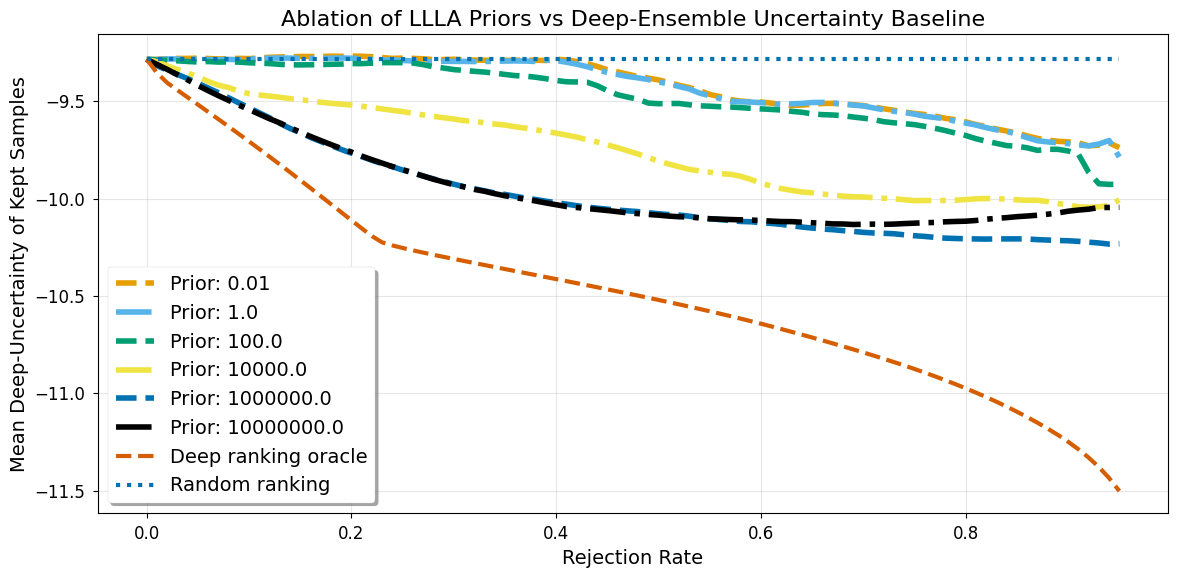
\includegraphics[width=0.9\linewidth]{figures/extend_toy/llla_prior_ablation.png}
    \caption{Ablation on $\gamma$ priors for \acs{LLLA}.  We observe the \acs{LLLA} improving by increasing the prior.}
    \label{fig:toy_gamma_ablation_prior}
\end{figure}

We do this for each \acs{LLLA}($\gamma$) ensemble to get the plot \autoref{fig:toy_gamma_ablation_prior}.

We see that higher $\gamma$ values improve performance until $10{,}000{,}000$. At very high $\gamma$, the influence of the \acs{NLL} Hessian vanishes, and the covariance converges to an isotropic matrix scaled by $1/\gamma$.

Conversely, lower, more reasonable $\gamma$ values yield severely degraded ensemble that fails at computing meaningful uncertainty values. To understand why reasonable $\gamma$ leads to failure, we must examine the specific geometry of our Toy network's loss landscape.

\begin{figure}[!htbp]
    \centering
    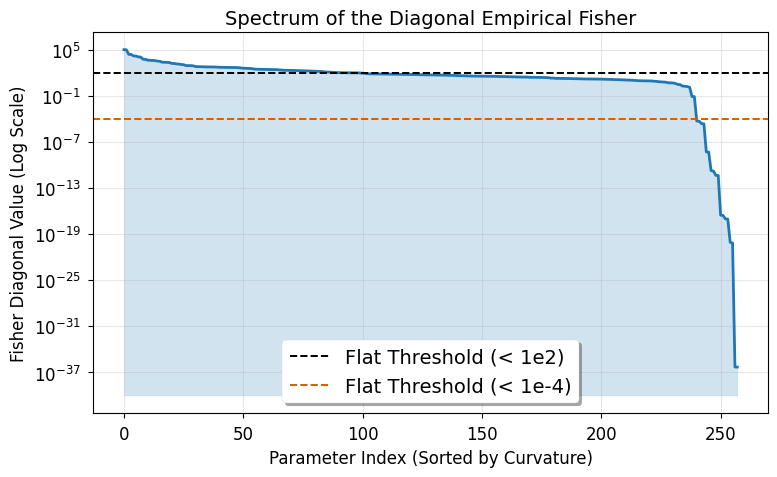
\includegraphics[width=0.8\linewidth]{figures/extend_toy/hessian_diag_values.png}
    \caption{Shows the diagonal values of the Hessian $H$ for each parameter of the last layer. The values are sorted and the scale is logarithmic.}
    \label{fig:hessian_diag_values}
\end{figure}

\paragraph{Analyzing the Hessian and Weights Space}
\autoref{fig:hessian_diag_values} shows us that although most Hessian diagonal values would be inverted fine and lead to a small jump in weight space, many would not. 
It's hard to tell exactly at what point Hessian values are big enough so that when inverted to give the covariance matrix, they lead to a sufficiently small jump in weight space for the \acs{LLLA} (2nd order Taylor approximation of the posterior in logarithm space) to stay valid. With \autoref{fig:toy_gamma_ablation_prior}, we can imagine needing to scale Hessian values up toward $10^6$ to reduce weight space jump to $10^{-6}$. By default the maximal Hessian value we have is $10^5$.

\paragraph{The High Prior Fix: ICLA}

\begin{figure}[!htbp]
    \centering
    \begin{subfigure}[b]{0.45\textwidth}
        \centering
        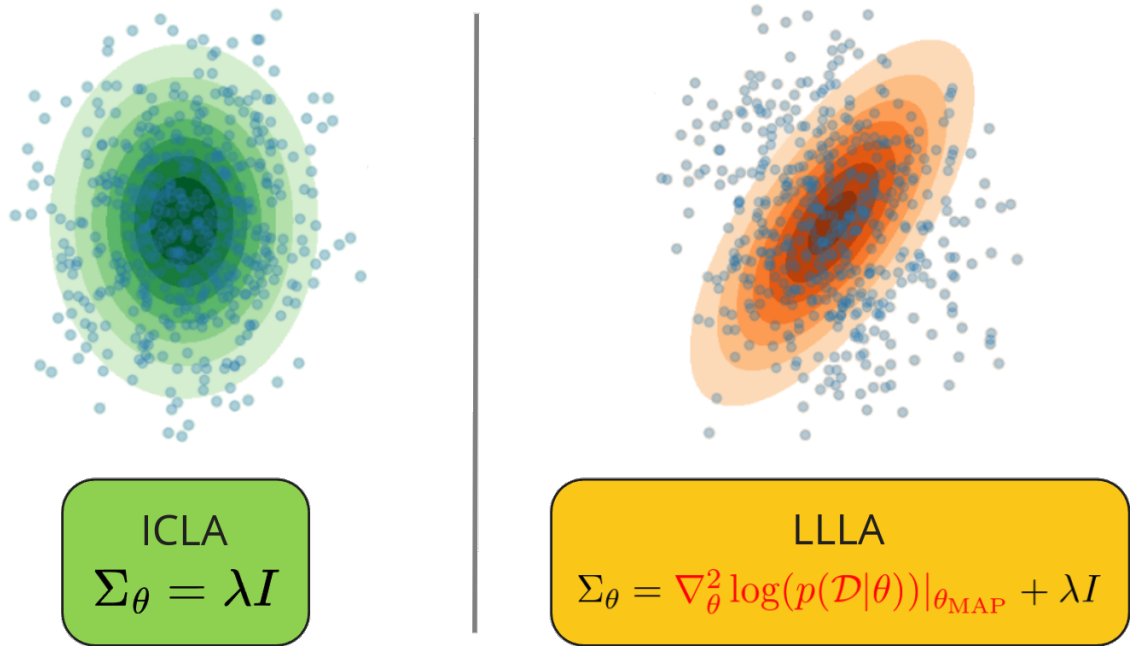
\includegraphics[width=\linewidth]{figures/extend_toy/icla.png}
        \caption{mathematical comparison between \acs{ICLA} and \acs{LLLA}. Note that $\Sigma_\theta = \lambda I = \frac{1}{\gamma} I$.}
        \label{fig:icla_vs_la}
    \end{subfigure}
     \hfill
    \begin{subfigure}[b]{0.45\textwidth}
        \centering
        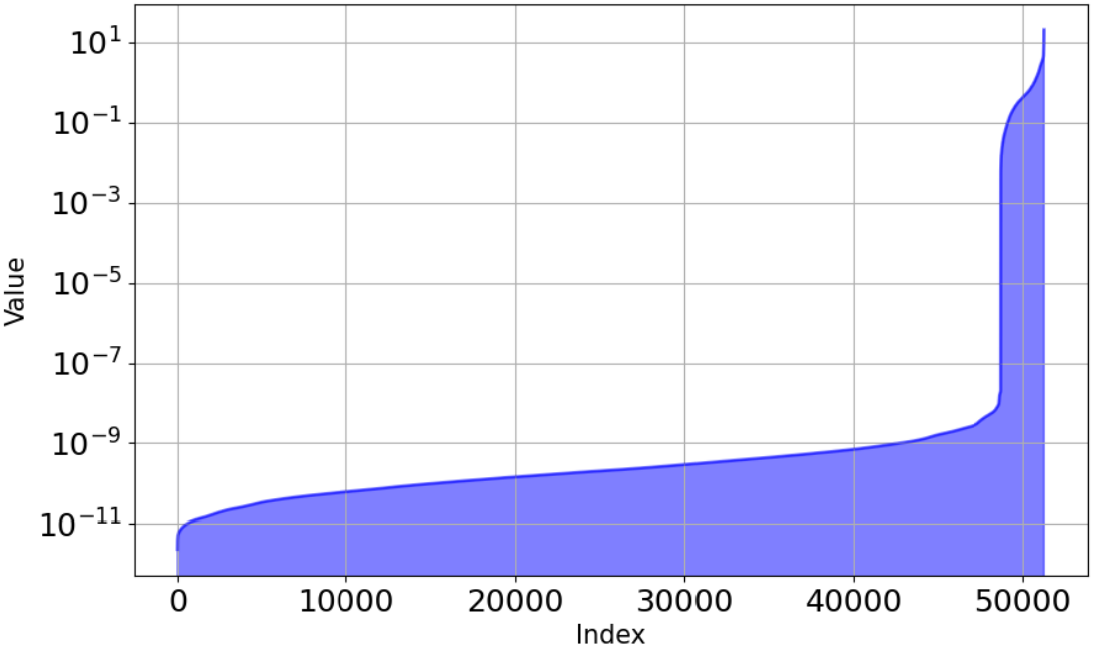
\includegraphics[width=\linewidth]{figures/extend_toy/icla_hessian_diag_values.png}
        \caption{Spectrum of Diagonal Fisher Values obtained in \parencite{zhdanov_identity_2024} \acs{LLLA} experiment.}
        \label{fig:icla_spectrum}
    \end{subfigure}
    \caption{Taken from \cite{zhdanov_identity_2024}.}
    % \caption{Taking the 4 most and least uncertain (w.r.t. \acs{GU}) images in a dataset 12032 generated images}
    \label{fig:icla_vs_la_and_spectrum}
\end{figure}

When we use such an high prior, we are effectively making the covariance matrix isotropic $\Sigma_\theta = H^{-1} = \frac{1}{\gamma}I$. This is actually not new in the literature and has been proven to sometimes even outperform the \acs{LLLA} \parencite{zhdanov_identity_2024}, here in the context of \acs{OOD} detection for natural images as well. In this paper however their spectrum of diagonal values of the Hessian was radically different from ours, they instead have a long tail of low fisher diagonal values with a spike at the end (\autoref{fig:icla_vs_la}). \cite{zhdanov_identity_2024} observed that having this long tail of low value with a spike of high values, leads to the \acs{ICLA} outperforming the \acs{LLLA}. Since in our case (\autoref{fig:hessian_diag_values}) we are in the exact opposite scenario, we hypothesize that we should be able to find use in the Hessian geometry instead of just making it isotropic.

\begin{tcolorbox}[colback=orange!10!white,colframe=orange!50!black,sharp corners]
Following what was said about using the \acs{MLE} instead of a \acs{MAP} trained model and the subsequent error made in the \acs{LA} that's growing with $\gamma$ (from \autoref{sub:la_trained_on_mle}), it could explain why only very high values of $\gamma$ actually work. Although the error in the \acs{LA} becomes massive, it does not matter since we are essentially ignoring the inverse Hessian computation of the log posterior in favor of an isotropic covariance matrix.
\end{tcolorbox}

\paragraph{Hallucinations Filtering}

\begin{figure}[!htbp]
    \centering
    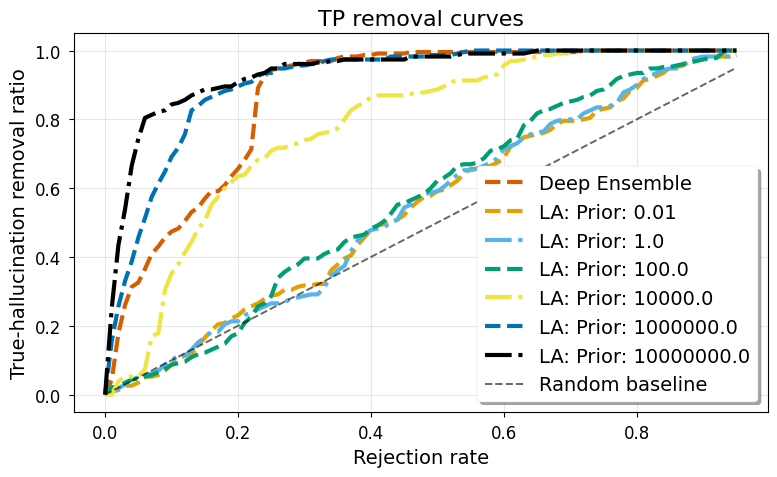
\includegraphics[width=0.8\linewidth]{figures/extend_toy/llla_prior_ablation_tp.png}
    \caption{Ratio of ``hallucinations'' removed as a function of Rejection rate with respect to the ensemble of models used to calculate uncertainty. Here we perform an ablation on the prior $\gamma$.}
    \label{fig:llla_prior_abla_tp}
\end{figure}

Before looking at ways to fix the Hessian values explosion while keeping the information it contains, let's look at a new metric that will help us differentiate \acs{LA} from \acs{DE} based ensemble.
We have only looked at how close we manage to get to the \acs{DE} baseline, but what happens if we instead look at how good an ensemble is at filtering ``\textit{hallucinations}'' defined as samples for which the $L2$ distance to the closest mode is bigger than $5\sigma$ (\autoref{sec:toy_what_gu_filter})\footnote{Although in the previous section we've used $6\sigma$, here we use $5 \sigma$, in practice it does not change much}. 

\begin{tcolorbox}[colback=gray!10!white,colframe=gray!50!black,sharp corners]
The idea of this metric is to measure the ratio of hallucinations we've successfully removed at any point in the filtering process.
\end{tcolorbox}

In \autoref{sec:toy_what_gu_filter}, what counts as ``hallucinations'' are both True Positives \textbf{TP} (what we were right to filter out) and False Negatives \textbf{FN} (what is left that we should filter out).

\begin{equation}
    TPR(r) = \frac{TP(r)}{TP(r) + FN(r)}
\end{equation}

Where $r$ is the rejection rate (the fraction of samples we filtered out already).
the metric gives us the ratio of identified hallucinations out of all hallucinations at the certain point $r$ in the filtering process.

\autoref{fig:llla_prior_abla_tp} shows us that higher prior \acs{LLLA} ($\simeq$ uniform diagonal covariance matrix) is better at filtering ``hallucinations'' than \acs{DE}. Looking closer, we see that \acs{DE} is eventually catching up but much later, this gap can be explained by the DE being able to filter out the full epistemic uncertainty (including samples that are valid but are associated to different modes across the $M+1$ models) (see \autoref{sec:toy_what_gu_filter}) while the \acs{LLLA} is blind to that part of uncertainty.

\subsection{The Temperature Fix} 

We've shown that \acs{ICLA} is an effective posterior approximation. But as explained previously from \parencite{zhdanov_identity_2024}, our Hessian values spectrum suggest that the Hessian geometry could actually be of use and should not be discarded.

Mathematically the \acs{LA} being a simple 2nd order approximation in logarithm space of the posterior distribution around the MAP estimator means that in the immediate neighborhood of $\theta_{MAP}$ the approximation holds. We have observed that the covariance matrix $\Sigma_\theta=H^{-1}$ lead to sampling models too far from $\hat\theta$, this suggests scaling the covariance matrix with a temperature parameter $T_s$, in our case, we are talking about the \acs{CPE} cold posterior effect with $T_s < 1$ and $\hat{\Sigma}_{\theta} = T_s^2 \Sigma_\theta$. Where $\Sigma_\theta$ is computed with a reasonable prior that preserves the Hessian geometry information while avoiding division by very small values.


\begin{figure}[!htbp]
    \centering
    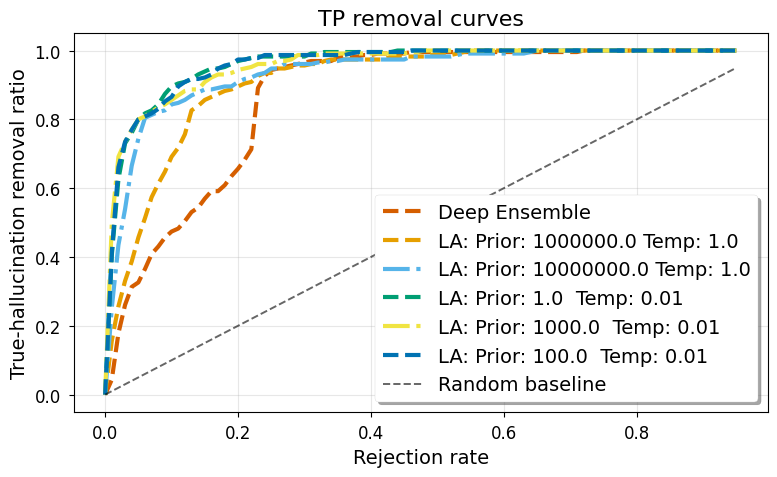
\includegraphics[width=0.8\linewidth]{figures/extend_toy/llla_temp_abla_tp.png}
    \caption{Ratio of Hallucinations as a function of Rejection rate, comparing the previous best $\gamma$ values with combinations of $\gamma$ and $T_s$.}
    \label{fig:llla_temp_abla_tp}
\end{figure}

\begin{figure}[!htbp]
    \centering
    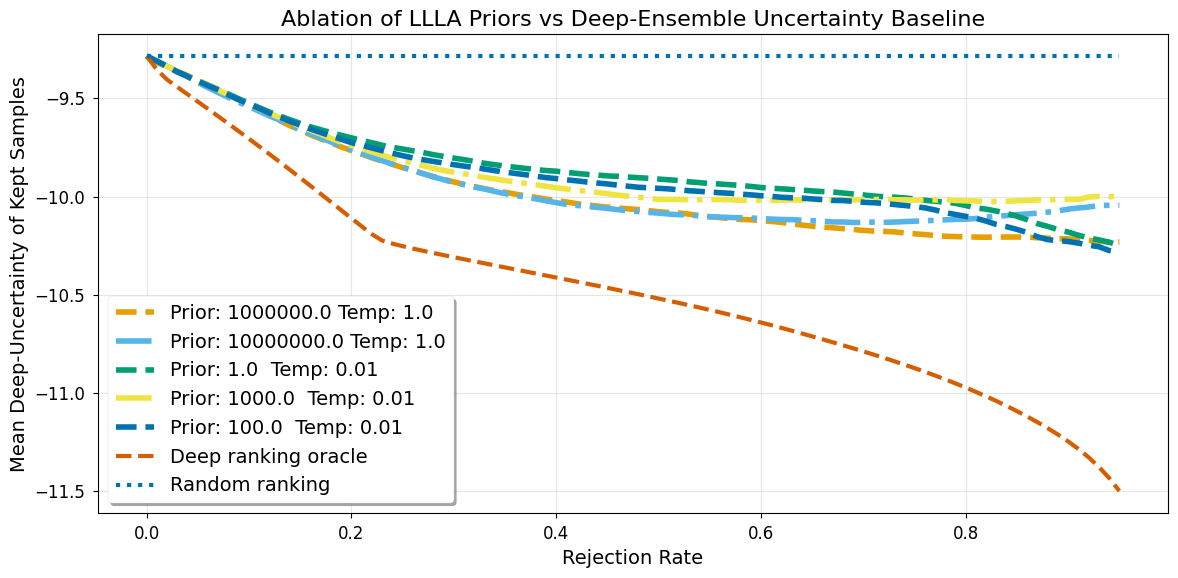
\includegraphics[width=0.9\linewidth]{figures/extend_toy/llla_temp_abla.png}
    \caption{Comparison of the previous best performing $\gamma$ values with combinations of $\gamma$ and $T_s$.}
    \label{fig:llla_temp_abla}
\end{figure}

We can indeed see on \autoref{fig:llla_temp_abla_tp} that lower priors can be better\footnote{It might seem like the $(\gamma, T)= (100.0,0.01)$ is not that much better than a very high prior like $10{,}000{,}000$ but actually this small change in rejection rate at which most ``hallucinations'' are removed translates to thousands of valid samples lost if we had just used the very high prior} at removing ``hallucinations'' than high priors provided we scale down the covariance matrix with a temperature parameter.
On the other hand, we can see on \autoref{fig:llla_temp_abla} that it is slightly worse on the Mean \acs{DE} metric.

We see next that we should not expect \acs{LLLA} or \acs{ICLA} to come close to \acs{DE} full epistemic uncertainty estimation anyway.



\section{Deep Ensemble vs Laplace Approximation}

\subsection{The Geometric Interpretation}
As observed in the Toy experiment, \acs{DE} seems to filter out samples where the ensemble members disagree on which mode the sample belongs to before starting to remove ``hallucinations''. This is expected because the distance between samples that are assigned to different modes is usually much bigger than the distance between samples assigned to the same mode but located too far from that mode. \acs{LA} instead directly targets ``hallucinations''.
This happens because \acs{DE} members are each fully trained from different random seeds, allowing them to settle into completely different low-loss basins. \acs{DE} therefore captures broad epistemic uncertainty, encompassing both off-mode samples and mode-assignment ambiguity. In contrast, the \acs{LA} is mathematically anchored to a local quadratic approximation around a single \acs{MAP} estimate. Because it is forced to take small steps within the same basin, it is functionally blind to model disagreement and naturally restricts its focus to off-mode perturbations.

\subsection{Superior performance of \acs{DE}}
% that single-basin methods cannot match the epistemic coverage of multi-basin exploration
This geometric limitation is rigorously quantified in  \cite{ashukha_pitfalls_2021}. In their uncertainty benchmark, they explicitly categorize the \acs{LLLA} (via the K-FAC Laplace Approximation) as a ``single-snapshot'' method inherently bound to a single mode of the loss landscape.

To measure the resulting performance gap, the authors introduced the Deep Ensemble Equivalent (\acs{DEE}) score, defined as ``What size of deep ensemble yields the same performance as a particular ensembling method?'' Their experiments revealed a severe inefficiency in local approximations: most single-snapshot methods (like \acs{LA}) require averaging predictions across dozens of samples $\mathrm{M}$, yet their predictive performance barely equates to an ensemble of only a few independently trained models.

Another big takeaway from \cite{ashukha_pitfalls_2021} was that temperature scaling is mandatory. Even though ensembles are generally better calibrated than single models, they are still not perfectly calibrated.
The \acs{DEE} is defined on the Calibrated Log-Likelihood (\acs{CLL}) model performance metric which is the log-likelihood evaluated after finding the optimal temperature post-hoc on a validation set.

The \acs{DEE} benchmark proves that the performance ceiling of \acs{LA} is fundamentally capped by its lack of mode diversity. This perfectly contextualizes our toy results: while our stabilized \acs{LLLA} is highly efficient at targeting severe hallucinations through local jittering, it structurally lacks the capacity to represent the full epistemic uncertainty required to match a \acs{DE}.

\subsection{What Do We Want to Filter Out?}

From everything we've seen in this toy experiment, there is no clear winner between \acs{LA} and \acs{DE}. Although \acs{DE} is sensible to the full uncertainty rather than just ``hallucinations'', it starts filtering the ``hallucinations'' late in the filtering process, whereas with \acs{LA} we can finish filtering out most ``hallucinations'' much earlier in the process \autoref{fig:llla_temp_abla_tp}. 

In the case of this toy experiment, if the aim is only to keep samples that belong to that gaussian mixture distribution, \acs{LLLA} is the clear winner. But in other applications like medical upscaling, we could imagine the model being unsure of ``which mode to choose'' to be equivalent to either make a tumor appear in the scaled image or not for instance, in which case \acs{DE} uncertainty would be absolutely mandatory to detect this kind of uncertainty. Still, this is quite speculative and should be tested with a proper experiment involving a more meaningful model as future work.

\subsection{A Bigger Picture (\acs{DE} + \acs{LLLA})}

One can also choose to combine the quick detection of hallucinations of \acs{LA} with the full uncertainty capability of \acs{DE}: \cite{eschenhagen_mixtures_2021} uses a mixture of both \acs{DE} and \acs{LLLA} (\acs{MoLA}) to get better results on multiple image classification benchmarks than \acs{DE}, Multi-\acs{SWAG} and many more.

\begin{figure}[!htbp]
    \centering
    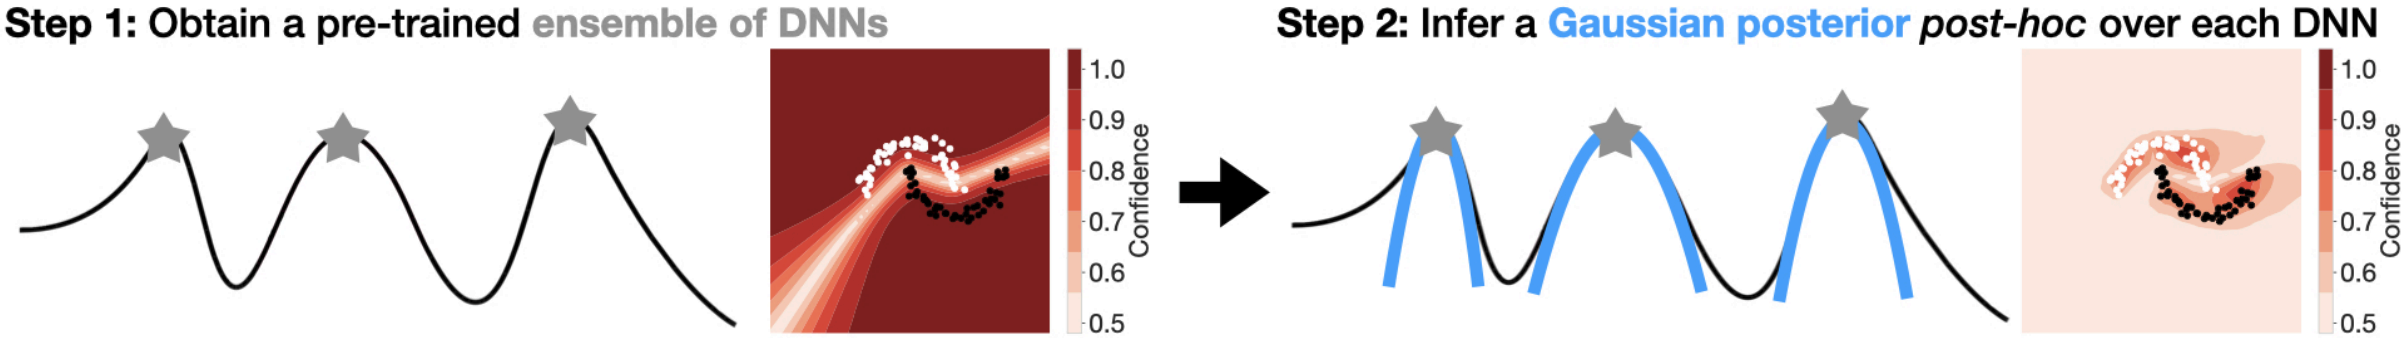
\includegraphics[width=0.9\linewidth]{figures/de_vs_la/de_vs_la.png}
    \caption{Taken from \cite{eschenhagen_mixtures_2021}, Illustrates the \acs{MoLA} method}
    \label{fig:de_vs_la}
\end{figure}

The \acs{LLLA} provides a deeper exploration of each basin found by \acs{DE}, \autoref{fig:de_vs_la}.


\section{What About the ADM Model ?}
\label{sec:what_about_adm}

First, does the prior ablation study results for the toy experiment translate to the ADM model? \cite{jazbec_generative_2025} conducted a similar ablation for $\gamma \in [0.01, 100.0]$ in their Appendix D and observed close to no changes to the \acs{FPR} metrics while doing so and in the end decided to set $\gamma=1$. 

One can observe in the Toy experiment \autoref{fig:toy_gamma_ablation_prior} that priors $\gamma$ in this range $[0.01, 100.0]$ give similar but really bad results. Though, the loss landscape and Hessian values spectrum could be very different between the Toy and \acs{ADM} Model, so this observation might not apply to the \acs{ADM} model. Still, in the next chapter (\autoref{ch:semantic-encoder}) we worryingly discover that the perturbation to the output made by the \acs{LLLA} might be equivalent to just adding random noise. 

To test if the \acs{LLLA} on the \acs{ADM} can be drastically improved the same way the Toy \acs{LLLA} was, we can run \autoref{ch:reproduce_adm} experiment with a low temperature scaling factor and/or much higher prior.

\begin{figure}[!htbp]
    \centering
    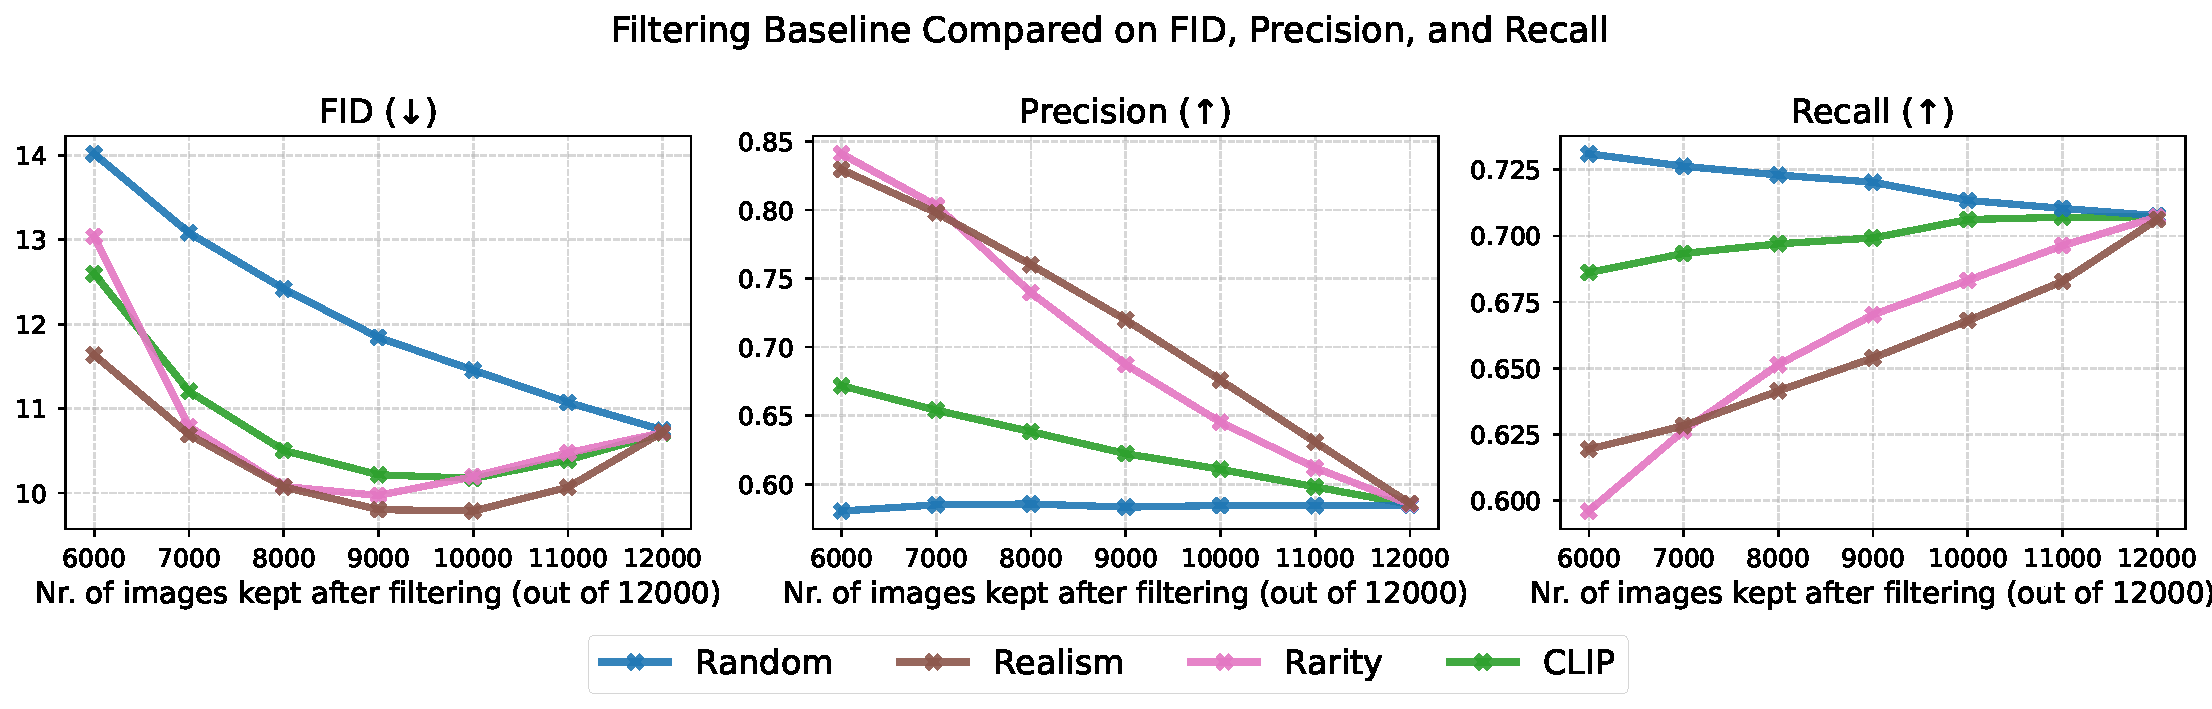
\includegraphics[width=0.95\linewidth]{figures/adm_temp/clip_temp_fpr.pdf}
    \caption{Reproduction of \autoref{ch:reproduce_adm} experiment with a temperature scaling factor of $T=0.01$}
    \label{fig:clip_temp_fpr}
\end{figure}

\autoref{fig:clip_temp_fpr} with $T=0.01, \gamma=1.0$ shows no improvement and looks even slightly worse than the results from \autoref{ch:reproduce_adm} which used $T=1.0, \gamma=1.0$.

Either the Hessian spectrum values of the \acs{ADM} are already scaled properly and we do not need any temperature scaling or high prior correction. Or as the next experiment suggest (\autoref{ch:semantic-encoder}), the posterior approximation is actually not the reason behind \cite{jazbec_generative_2025} \acs{ADM} uncertainty measurement performance on the \acs{FPR} metrics and improvements can therefore not be measured this way. 

\section{Conclusion}

In conclusion, we've shown that \acs{LLLA} can actually perform well in the context of a Toy diffusion model contrary to what was previously thought in \cite{gupta_quantifying_2026} for instance, provided we play around with high priors or temperature scaling.
